\documentclass[aspectratio=169, t, 10pt]{beamer}
\usetheme{Boadilla}
\beamertemplatenavigationsymbolsempty

\usepackage{standalone}
\usepackage[utf8]{inputenc}
\usepackage[english]{babel}
\usepackage{pgfplots}
\usepackage{mathtools}
\mathtoolsset{showonlyrefs}
\usepackage{qrcode}
\usepackage{multimedia}

\newcommand\Mean[1]{\mathbb{E}\!\left[#1\right]}
\newcommand\Var[1]{\mathbb{V}\!\left[#1\right]}
\newcommand\Cov[2]{\mathrm{Cov}\!\left[#1,#2\right]}
\newcommand\Gauss[2]{\mathcal{N}\!\left({#1},\,{#2}\right)}
\newcommand\GP[2]{\mathcal{GP}\!\left({#1},\,{#2}\right)}
\newcommand{\Identity}{\mathbb{I}}

\title[Correlation based travel time inversion]{Bayesian Travel Time Inversion adopting Gaussian Process Regression}
\subtitle{-- with the focus on uncertainty analysis --}
\author[\tt mauerber@uni-potsdam.de]{Stefan Mauerberger \and Matthias Holschneider}
\institute[Math@UP]{University Potsdam, Institute of Mathematics}
\titlegraphic{%\vspace{-1cm}
              \hspace{2cm}
              \parbox[c]{0.17\linewidth}{
\includegraphics[width=\linewidth]{./logos/GeoSim_Logo}}
              \hfill
              \parbox[c]{0.10\linewidth}{
\includegraphics[width=\linewidth]{./logos/UniPotsdam_Logo}}
              \hspace{2cm}
              }
\date[AGU~2017]{AGU Fall Meeting -- 13\textsuperscript{th} December 2017}

\begin{document}
\input{def_example}

\frame[noframenumbering, plain]
    {\maketitle}

\begin{frame}
    \frametitle{Correlation-Based Bayesian Tomography}
    \framesubtitle{A non-parametric approach (function space veiw)}

\begin{columns}%
\column{.55\textwidth}%

    \begin{exampleblock}{Setting \& Simplifications}
        \begin{itemize}
            \item Proof of concept
            \item Synthetic test
            \item Neglecting dispersion and refraction
            \item Reference model: Two large scale anomalies
            \item Pseudo observations corrupted by normal noise
        \end{itemize}
        \hfill {\Large $\leadsto$} Location dependent model uncertainties ~
    \end{exampleblock}


\column[T]{.44\textwidth}
    \vspace{-10mm}
    \only<1>{\input{fig_reference_model.pgf}}
    \only<2>{\input{fig_reference_model_cnt.pgf}}
\end{columns}

\end{frame}

\begin{frame}
    \frametitle{Travel Time Observations}
    \framesubtitle{a functional w.r.t.~the velocity model}

\begin{columns}
\column{.55\textwidth}%
    \begin{equation}
        d = \mathrm T_{s,r}[v] + \varepsilon = \int_C \frac 1{v(r)} \mathrm d r + \varepsilon
    \end{equation}
    @Matthias: This is a Radon transformation, am I right?
    \begin{description}[leftmargin=! ,labelwidth=1cm]
        \item [Measured value]           $d$
        \item [Observational functional] $\mathrm T_{s,r}[\cdot]$
        \item [Source location]          $s$
        \item [Receiver position]        $r$
        \item [Velocity model]           $v$
        \item [Measurement error]        $\varepsilon$
        \item [Ray path]                 $C$
    \end{description}

    \begin{alertblock}{It is the velocity model what we are after}
    \begin{itemize}
        \item Travel times are putting an Integral-constraint on $v$
        \item Non-linearity is a major concern
    \end{itemize}
    \end{alertblock}


\column[T]{.44\textwidth}
    \vspace{-10mm}
    \only<1>{\input{fig_path_coverage.pgf}}
    \only<2>{\input{fig_discretization.pgf}}
    \small
    \begin{align}
        N_\text{stn} &= \SFWnst &
        & \leadsto &
        N_\text{obs} &= \SFWnobs
        \\
        \onslide<2>{
            \delta\sphericalangle &\approx \SFWdeltaangle\,^\circ &
            & \leadsto &
            N_\text{grd} &= \SFWnpts
        }
    \end{align}

\end{columns}

\end{frame}


\begin{frame}
    \frametitle{A\,Priori Velocity Model}
    \framesubtitle{expressing our ignorance}

\begin{columns}
\column{.55\textwidth}%
    \begin{block}{Model $v(x)$ a Gaussian Random Field}
    \begin{equation}
        v \to V \sim \GP{\mu_V}{K_V}
    \end{equation}
    \begin{description}[leftmargin=! ,labelwidth=6cm]
        \item [Prior mean function] $\mu_V(x) = \SFWmuCpri \, \frac ms$
        \item [Covariance function] $K_V(x,y)$
    \end{description}
    \end{block}
    \medskip

    Assumed covariance
    \begin{equation}
        K_V(x,y) = \tau^2 \exp\left\{ -\frac12 \frac{d(x,y)^2}{\ell^2}\right\}
    \end{equation}
    \begin{description}[leftmargin=! ,labelwidth=6cm]
        \item [Great circle distance] $d(x,y)$
        \item [Standard deviation]   $\tau = \SFWtau \, \frac ms$
        \item [Characteristic lenth]  $\ell = \SFWell \, m$
    \end{description}

\column[T]{.44\textwidth}
    \vspace{-10mm}
    \input{fig_kernel_pri.pgf}

\end{columns}

\end{frame}


\begin{frame}
    \frametitle{Linearization}
    \framesubtitle{Gaussianity is only preserved under linear maps}

\begin{columns}
\column{.55\textwidth}%
    \begin{equation}
        \mathrm T_{s,r}[V] \approx \int_C \frac 1{\mu_V(r)} - \frac{V(r)}{\mu_V(r)^2} \mathrm d r
    \end{equation}
    \begin{description}[leftmargin=!, labelwidth=1cm]
        \item [Taylor expansion] 1\textsuperscript{st} order
        \item [point of expansion] $\mu_V$ (prior mean)
    \end{description}
    \medskip

    \begin{block}{Approximated correlations}
    \begin{equation}
        \Cov{V}{\mathrm T_{s,r}[V]\,} \approx -\int_C \frac {K_V(\cdot,r)}{\mu_V(r)^2} \mathrm d r
    \end{equation}
    \end{block}

    \begin{block}{Approximated covariance}
    \setlength\abovedisplayskip{0pt}
    \begin{equation}
        \Cov{\mathrm T_{s,r}[V]}{\mathrm T_{\acute s, \acute r}[V]\,} \approx  \int_C \int_{\acute C} \frac{K_V(r,\acute r)}{\mu_V(r)^2\mu_V(\acute r)^2} \mathrm d r \mathrm d \acute r
    \end{equation}
    \end{block}

\column[T]{.44\textwidth}
    \vspace{-10mm}
    \input{fig_correlation_pri.pgf}%
    \vspace{-2mm}
    \begin{center}%
    \small Correlation of $V(x)$ with $T_{s,r}[V]$ kept fix
    \end{center}

\end{columns}

\end{frame}


\begin{frame}
    \frametitle{Bayesian Posterior Distribution}
    \framesubtitle{Gaussian Process Regression}

\begin{columns}
\column[t]{.48\textwidth}

    \begin{block}{Stochastic data model}
        \begin{equation}
            D = \mathrm T_{s,r}[V] + E \sim \Gauss{\mu_D}{\Sigma_{DD}}
        \end{equation}
        \begin{description}[labelwidth=25mm]
            \item [Error model]        $E\sim \Gauss{0}{\sigma_\varepsilon^2}$
            \item [Uncertainty]        $\sigma_\varepsilon = \SFWepsilon\,s$
            \item [Prior travel times] $\mu_D = \Mean{\mathrm T_{s,r}[\mu_V]\,}$
            \item [Covariance matrix]  $\Sigma_{DD} = \Cov{\mathrm T}{\mathrm T}  + \Identity \sigma_\varepsilon^2$
        \end{description}
    \end{block}

    \begin{itemize}
        \item The kernel spans a function space (RKHS)
        \item Sort out functions incompatible with data
    \end{itemize}

\column[t]{.48\textwidth}

    \begin{exampleblock}{Conditional mean and covariance}
        \setlength\abovedisplayskip{0pt}
        \begin{alignat}{3}
            \Mean{V|d} &= \mu_V &&+ \Cov VD \Sigma_{DD}^{-1} \big( d - \mu_{D} \big)
            \\
            \Var{V|d}  &= K_V   &&- \Cov VD \Sigma_{DD}^{-1} \Cov DV
        \end{alignat}
        \hfill {\Large $\leadsto$} Posterior distribution \phantom{p}
    \end{exampleblock}

    \begin{alertblock}{Accommodate non-linearity}
        \begin{itemize}
            \item Single evidence at a time
            \item Correlations and Variances from predecessor
        \end{itemize}
        \hfill {\Large $\leadsto$} Successive approach ~
    \end{alertblock}

\end{columns}

\end{frame}


\begin{frame}
    \frametitle{Successive Approach}
    \begin{center}
    \movie[height=0.85\textheight, width=1.51\textheight, autostart]{\includegraphics[height=0.85\textheight, width=1.51\textheight]{animation_pst}}{animation.avi}
    \end{center}
\end{frame}


\begin{frame}
    \frametitle{Posterior Correlation Pattern}
    \framesubtitle{\dots }

\begin{columns}
\column{.55\textwidth}%
    \begin{itemize}
        \item Analogy with sensitivity kernel
    \end{itemize}

\column[T]{.44\textwidth}
    \vspace{-10mm}
    \only<1>{\input{fig_correlation_pri.pgf}}
    \only<2>{\input{fig_correlation_pst.pgf}}

\end{columns}

\end{frame}


\begin{frame}
    \frametitle{Conclusions}
    \framesubtitle{Preliminary results}

\begin{columns}
\column{.55\textwidth}%

    \begin{itemize}
        \item Accounts for irregular data distributions
        \item Linearization performs well
        \item Realistic assessment of spatial uncertainties
        \item Computationally simple
        \item All calculus in the function space view \\
              No basis functions, no truncations at a certain degree
        \item Memory intense
        \item Succession order
    \end{itemize}

\column[T]{.44\textwidth}
    \vspace{-5mm}
    \begin{tikzpicture}
        \pgfplotstableread{./dat/misfit.dat}\misfit
        \begin{semilogyaxis}[width=\textwidth, height=0.9\textheight,
                 label={Data misfit}, xlabel={\# evidence},
                 axis lines=left, legend cell align=left,
                 tick label style={font=\scriptsize}, legend style={only marks, draw=none, font=\footnotesize},
                 label style={font=\scriptsize}, log ticks with fixed point ]
            \addplot [dashed, mark=*, blue , mark options={scale=0.5, solid}] table [x=evd, y=all] \misfit;
            \addlegendentry{all at once}
            \addplot [dashed, mark=*, red  , mark options={scale=0.5, solid}] table [x=evd, y=asc] \misfit;
            \addlegendentry{ascending $\sphericalangle$}
            \addplot [dashed, mark=*, green, mark options={scale=0.5, solid}] table [x=evd, y=dsc] \misfit;
            \addlegendentry{descending $\sphericalangle$}
            \addplot [dashed, mark=*, black, mark options={scale=0.5, solid}] table [x=evd, y=rnd1] \misfit;
            \addlegendentry{shuffle}
            \addplot [dashed, mark=*, black, mark options={scale=0.5, solid}] table [x=evd, y=rnd2] \misfit;
        \end{semilogyaxis}
    \end{tikzpicture}

\end{columns}

\end{frame}

\begin{frame}[c]
    \frametitle{Outlook \& Next Steps }
    \framesubtitle{Potential future application}

\begin{columns}
\column{.55\textwidth}%


    \begin{block}{Surface Wave Tomography}
        \begin{itemize}
            \item Ambient noise records
            \item Model phase velocities $v(\omega)$
            \item A frequency dependent kernel
                \begin{equation}
                    K(x,\omega; \acute x, \acute\omega) \overset{?}{=}
                    \tau(\bar \omega)^2 \exp\left\{ -\frac12 \frac{\|x - \acute u\|^2}{\ell(\bar \omega)^2}\right\}
                \end{equation}
                to account for dispersion
            \item Estimation of hyper parameters
        \end{itemize}
    \end{block}

\column[T]{.44\textwidth}
    \only<1>{
    \vspace{-10mm}
    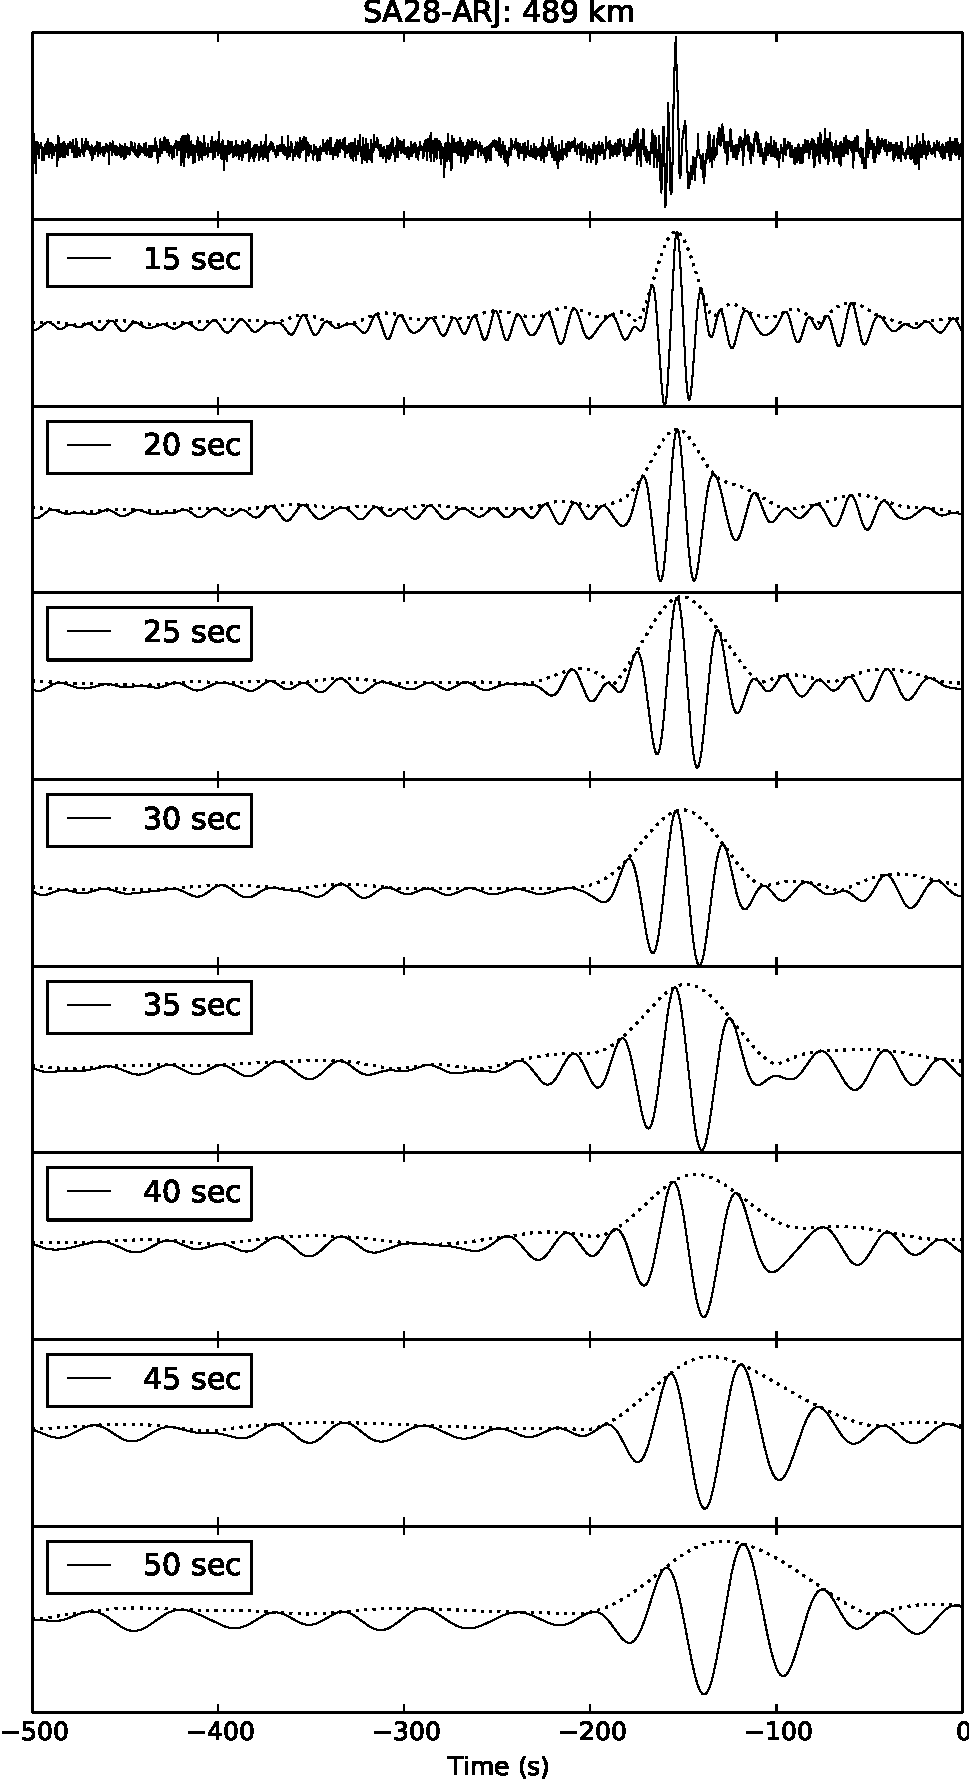
\includegraphics[height=0.95\textheight]{MultiFiltered_SA28-ARJ}
    }
    \only<2>{
    \vspace{-6mm}
    \begin{center}
        Follow the project on GitHub
        \\[6mm]
        \fbox{\qrcode[height=3cm]{https://github.com/mauimuc/gptt}}
        \\[6mm]
        \small
        \href{https://github.com/mauimuc/gptt}{github.com/mauimuc/gptt}
    \end{center}
    }
\end{columns}

\end{frame}

\end{document}
